% ============================================================
%  深圳大学实验报告（基于 Experiment-Report-Template-SZU）
%  项目：NumPy 复现 OpenCLIP 图像编码器
%  编译：XeLaTeX
% ============================================================
\documentclass[a4paper,12pt]{article}

\usepackage{fontspec}
\usepackage{xeCJK}
\setCJKmainfont{Noto Serif CJK SC}
\usepackage{geometry}
\geometry{left=1in, right=1in, top=1in, bottom=1in}
\usepackage{longtable}
\usepackage{graphicx}
\usepackage{fancyhdr}
\usepackage{tikz}
\usetikzlibrary{calc}
\usepackage{verbatim}
\usepackage{float}
\usepackage{xcolor}

\fancyhf{}

\begin{document}

% ==================== 封面 ====================
\begin{titlepage}
    \centering
    \vspace*{2cm}
    \Huge{\textbf{深 \ 圳 \ 大 \ 学 \ 实 \ 验  \ 报 \ 告}}\\[1.5cm]
    {\Large\textbf{课程名称}\quad\underline{\makebox[8cm][c]{Python 程序设计}}}\\[0.5cm]
    {\Large
    \noindent\makebox[3.2cm][l]{\textbf{项目名称}}
    \underline{\makebox[8cm][c]{NumPy 复现图像编码器}}}\\[0.5cm]
    {\Large
    \noindent\makebox[3.2cm][l]{\textbf{学 \quad \quad 院}}
    \underline{\makebox[8cm][c]{人工智能学院}}}\\[0.5cm]
    {\Large
    \noindent\makebox[3.2cm][l]{\textbf{专 \quad \quad 业}}
    \underline{\makebox[8cm][c]{}}}\\[0.5cm]
    {\Large
    \noindent\makebox[3.2cm][l]{\textbf{指导教师}}
    \underline{\makebox[8cm][c]{舒婷}}}\\[0.5cm]
    {\Large
    \noindent\makebox[3.2cm][l]{\textbf{报 \quad 告 \quad 人}}
    \underline{\makebox[3cm][c]{}}
    \hspace{0.5cm}
    \textbf{学号}
    \underline{\makebox[3cm][c]{}}}\\[0.5cm]
    {\Large
    \noindent\makebox[3.2cm][l]{\textbf{实验时间}}
    \underline{\makebox[8cm][c]{}}}\\[0.5cm]
    {\Large
    \noindent\makebox[3.2cm][l]{\textbf{提交时间}}
    \underline{\makebox[8cm][c]{}}}\\[1.5cm]
    \vfill
    \Large{\textbf{教务处制}}
\end{titlepage}
\newpage

% ==================== 正文 ====================
\section{实验目的}

本实验要求仅用 NumPy 复现 OpenCLIP ViT-B-32 \emph{图像编码器}的前向计算：
给定预处理后的图像张量 $[B,3,224,224]$ 与随附的训练权重，逐层算出每张图的
512 维单位向量 $[B,512]$，并在数值上与随附的独立 FP32 参考对齐。该编码器即期末
项目图像塔的接口预演，不需要任何训练。通过本实验掌握：图像分块（patchify）、
多头自注意力、前馈网络、残差与层归一化的数值实现，以及权重存储布局
$[out,in]$ 与矩阵乘方向的关系。

\section{方案概述}

整体流程如图~\ref{fig:pipeline} 所示，分为六个必须补全的任务（红色标注为评分要求的
实现部分）。输入图像先切成 $7\times7=49$ 个 $32\times32$ 的 patch（TODO-01），
线性投影到 768 维并在最前面拼接一个可学习的 CLS token、加上位置编码（TODO-05），
得到 $[B,50,768]$ 的 token 序列。随后经过 12 个结构相同的 Transformer block
（TODO-02/03/04，形状不变），最后取 CLS 行、后归一化、投影到 512 维并单位化
（TODO-06）得到输出。

\begin{figure}[H]
    \centering
    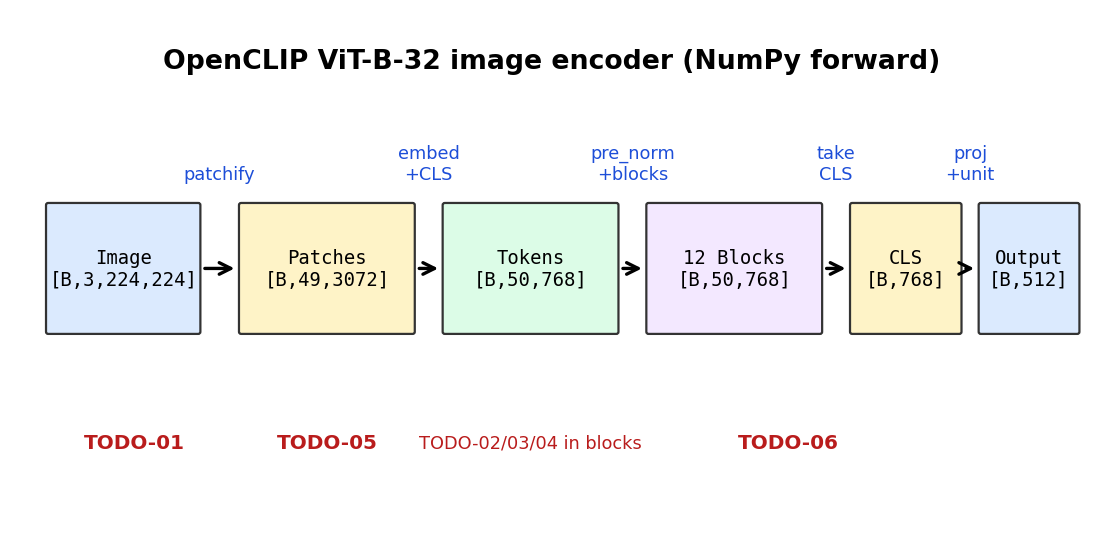
\includegraphics[width=0.94\linewidth]{figs/pipeline.png}
    \caption{图像编码器整体流水线。红色标注为需要补全的 TODO 代码要求部分。}
    \label{fig:pipeline}
\end{figure}

\section{关键实现}

\subsection{TODO-01：patchify 的轴变换}

把 $[B,3,224,224]$ 变为 $[B,49,3072]$ 的核心是 reshape--transpose--reshape。
先把 $224$ 拆成 $7\times32$（7 个 patch，每块 32 像素），得到
$[B,3,7,32,7,32]$，轴序为 $B,C,g_h,p_h,g_w,p_w$；再用
\texttt{transpose(0,2,4,1,3,5)} 调成 $B,g_h,g_w,C,p_h,p_w$；最后把
$(g_h,g_w)$ 合并成 49、$(C,p_h,p_w)$ 合并成 3072（图~\ref{fig:patch}）。

\begin{figure}[H]
    \centering
    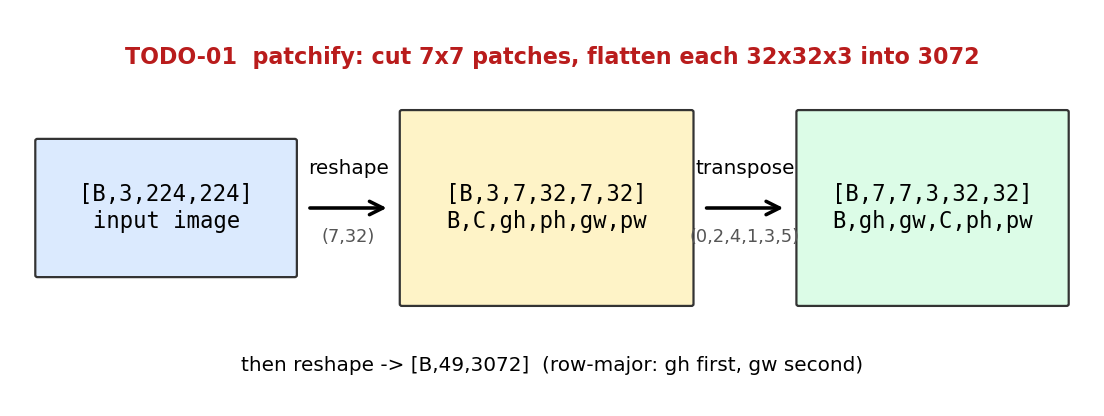
\includegraphics[width=0.94\linewidth]{figs/patchify.png}
    \caption{TODO-01 的 reshape 与 transpose 轴重排过程。}
    \label{fig:patch}
\end{figure}

\subsection{TODO-03/04：多头注意力与 Transformer block}

单个 block 的结构如图~\ref{fig:block}。注意力分支：由 $x$ 经三个线性投影得到
$q,k,v$，切分为 12 个头（每头 64 维）；分数为
$\mathrm{scores}=qk^{\top}/\sqrt{64}$，经逐行 softmax 得系数后加权求和 $v$，
合并 12 个头再过输出投影（TODO-02/03）。这里 $k$ 是四维
$[B,H,N,64]$，只能交换最后两轴 \texttt{swapaxes(-1,-2)}，不能用 \texttt{k.T}。

\begin{figure}[H]
    \centering
    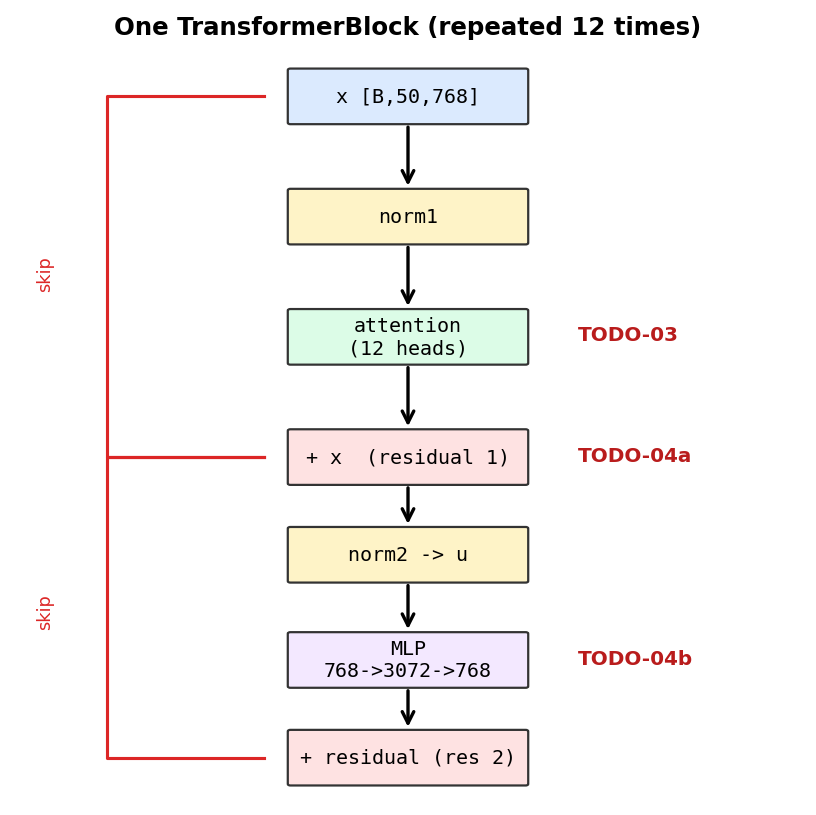
\includegraphics[width=0.62\linewidth]{figs/block.png}
    \caption{单个 Transformer block：两条残差路径（红色）与 TODO 位置。}
    \label{fig:block}
\end{figure}

MLP 分支：对每个 token 做
$\mathrm{GELU}(uW_1^{\top}+b_1)W_2^{\top}+b_2$，中间层扩到 3072 维再压回 768。
两个子层各自以残差方式加回主干（TODO-04a/04b）。注意所有线性权重都按
$[out,in]$ 存储，必须转置；GELU 用提供的精确 \texttt{erf} 版本，Norm 的
$\varepsilon=10^{-5}$，全程 float32。

\subsection{TODO-06：输出}

取第 0 个 token（CLS）：$[B,50,768]\rightarrow[B,768]$，经 \texttt{post\_norm}
后乘 \texttt{self.projection}（$[768,512]$，已是 $[in,out]$，\textbf{不转置}）得
$[B,512]$，最后 \texttt{unit\_vector} 归一化为单位向量。

\section{实验结果}

用参考中已预处理好的图像直接驱动编码器，逐阶段与独立 FP32 参考比较，结果如表~\ref{tab:err}：
所有阶段通过，输出最大绝对误差在 $10^{-6}$ 量级，单位向量模长偏差约 $1.2\times10^{-7}$。
乱序加重复的 batch 检查同样通过，说明实现可处理任意 batch。

\begin{table}[H]
\centering
\caption{各阶段数值误差（正确预处理输入）。}
\label{tab:err}
\begin{tabular}{l c c}
\hline
阶段 & 最大绝对误差 & 结果 \\
\hline
patches     & 0.000e+00 & PASS \\
tokens      & 4.578e-05 & PASS \\
block0      & 6.348e-06 & PASS \\
last\_tokens& 4.482e-05 & PASS \\
output      & 6.258e-07 & PASS \\
batch       & 4.321e-07 & PASS \\
\hline
\end{tabular}
\end{table}

\section{讨论}

\emph{一个形状变化}：MLP 把 token 从 768 维临时扩展到 3072 维（$4\times$ 隐藏层），
经 GELU 后再压回 768，因此 block 的输入输出形状始终为 $[B,50,768]$，这是 12 层
可以直接堆叠的原因。

\emph{一个修复的 bug}：初版 MLP 写成 \texttt{u @ self.fc1\_weight}，
由于权重形状为 $[3072,768]$，与 $u$ 的最后一维 768 不匹配，运行时报矩阵维度错误。
改为 \texttt{u @ self.fc1\_weight.T}（\texttt{fc2} 同理）后通过。根因是线性权重按
$[out,in]$ 存储，矩阵乘必须右乘其转置。

\emph{已知环境问题}：本机 Pillow 11.0.0 的 bicubic resize 与生成参考时的版本不同，
使 \texttt{check.py} 的 \texttt{preprocess} 阶段报 FAIL，并连带后续阶段；这是输入
预处理差异而非编码器错误，用正确预处理输入验证时全部 PASS。

\section{贡献与说明}

本报告中编码器六个 TODO 的实现、示意图绘制、数值验证与文档撰写由本人完成；
课程提供的权重、参考数据、\texttt{helpers.py}、\texttt{preprocess\_image.py}、
\texttt{run.py}/\texttt{check.py}/\texttt{runtime.py} 未作修改。实现过程中参考了课程
课件与 \texttt{PPT-CODE-MAP.txt} 的代码映射；报告模板来自深圳大学实验报告
Overleaf 模板。未使用生成式模型代替实现本身，仅用其辅助文字整理。

\newpage

% ==================== 批阅与成绩评定页 ====================
\begin{tikzpicture}[remember picture, overlay]
  \draw[thick]
    ($(current page.north west)+(2cm,-3cm)$)
    rectangle
    ($(current page.south east)+(-2cm,3.5cm)$);
\end{tikzpicture}

\vspace{1cm}
\noindent \textbf{指导教师批阅意见：}
\vspace{6cm}
\hfill

\vspace{1cm}
\noindent \textbf{成绩评定：}
\vspace{2cm}
\hfill

\vspace{1cm}
\noindent
\hfill
\textbf{指导教师签字：}\quad\quad\quad\quad\quad\\[0.5cm]
\hfill
\textbf{年}\quad\quad
\textbf{月}\quad\quad
\textbf{日}\quad

\vspace{1cm}
\noindent \textbf{备注：}

\begin{tikzpicture}[remember picture, overlay]
  \node[
    anchor=north west,
    inner sep=0pt,
    text width=\dimexpr\paperwidth-4cm\relax
  ] at ($(current page.south west)+(2cm,3.1cm)$) {
    \begin{minipage}{\dimexpr\paperwidth-4cm\relax}
      \small
      \noindent
      \textbf{注：}\;1、报告内的项目或内容设置，可根据实际情况加以调整和补充。\\[0.2cm]
      \phantom{\textbf{注：}\;}2、教师批改学生实验报告时间应在学生提交实验报告时间后 10 日内。
    \end{minipage}
  };
\end{tikzpicture}

\end{document}
